\section{Evaluation}
\label{sec:evaluation}

This section describes how we evaluated our model through two case studies of existing software development security data.

We presented the data elements to be collected for our full model in Section ~\ref{sec:model_measurement}, and the data collection guide for the measurement model gives instructions on how to collect the data for a software development project~\cite{morrison2016spefsite}.  SEM is a large-sample technique, with median sample size in the literature of 200 cases~\cite{kline2015principles}. The need for large quantities of software development security data leads us to examine existing software development security datasets. In addition to the practical considerations of requiring large amounts of data, confirmation of our hypothesized structural and measurement relationships in data we did not author would strengthen the case for the theorized relationships.
We have identified two candidate data sets, of increasing detail and decreasing observation count: 
\begin{itemize}
\item The National Vulnerability Database contains vulnerability records for a wide variety of software, over a long timespan.
\item The Core Infrastructure Initiative project census contains high-level project data for over 400 Debian~\footnote{https://www.debian.org/} packages.
\end{itemize}

We give further details for each of these datasets in their case study sections, below. We used the R~\footnote{https://www.r-project.org}  lavaan~\cite{roseel2012lavaan} (LAtent VAriable ANalysis) package to conduct our SEM analysis, as well as the ggplot2, semPlot and psych R packages.

\subsection{National Vulnerability Database Case Study}
\label{sec:evaluation_nvd}
The U.S. National Institute of Standards and Technology (NIST) maintains the National Vulnerability Database (NVD) ~\footnote{https://nvd.nist.gov/}, an online database of publicly reported software vulnerabilities, with over 79,000 vulnerabilities dating back to 1988. Vulnerability reporters assign each vulnerability a Common Vulnerability Scoring System (CVSS) score and associated CVSS base metrics, according to the scheme defined in the CVSS guide~\cite{mell2007complete}.  

\subsubsection{Data selection}
\label{sec:evaluation_nvd_selection}
 We translate the CVSS metrics into the terms of our model constructs and measurements. For each structural model construct, we present our metric associations and the rationale behind them.
 
\textbf{Asset Value}
The CVSS Confidentiality Impact, Integrity Impact, and Availability Impact metrics measure the degree of loss of confidentiality, integrity, and availability represented by a reported vulnerability~\cite{mell2007complete}. The CVSS Impact values:
	\begin{itemize}
		\item 'None' indicates no impact, 
		\item 'Partial' indicates partial impact, and 
		\item 'Complete' indicates 'Complete' impact to the CIA property of the system by the exploited vulnerability.  
	\end{itemize}
We model each Impact metric as a component of Asset Value, theorizing that confidentiality, integrity, and availability impacts change based on the usage context in which the software is run, e.g. the value of the assets managed. We translate None/Partial/Complete to an ordinal scale to model increasing CIA impact risk.

\textbf{Software Risk}
\label{sec:evaluation_nvd_selection_risk}
The CVSS Access Vector, Access Complexity, and Authentication metrics capture how a vulnerability is accessed and whether or not extra conditions are required to exploit it.~\cite{mell2007complete}. We translate these metrics into the terms of our model constructs and measurements. For each metric, we now quote the CVSS guide definition, and give a rationale for the associations we have defined:
\begin{itemize}
	\item Access Vector - measures how the vulnerability is exploited, in terms of network distance. Values:
	\begin{itemize}
		\item 'Local' requires the attacker to have physical access or an account on the system, \item 'Adjacent Network' requires access to the physical network on which the vulnerable software resides, and \item 'Network' requires only logical network acccess, e.g. remote access. 
	\end{itemize}
	We model Access Vector Risk as a component of Software Risk, theorizing that the vector value changes based on design choices made by the software development team. We translate the CVSS Access Vector values to an ordinal scale to model increasing `Access Vector Risk'.
	\item Access Complexity - measures the complexity of attack required to exploit a vulnerability once an attacker has gained access. Values: 
	\begin{itemize}
		\item 'High' indicates specialized/elevated access is required to exploit the vulnerability, 
		\item 'Medium' indicates that some access is required to exploit the vulnerability, and \item 'Low' indicates that the vulnerability can be exploited with default/no special access.  
	\end{itemize}
	We model Access Complexity Risk as a component of Software Risk, theorizing that the complexity value changes based on design choices made by the software development team. We translate the CVSS Access Complexity  to an ordinal scale to model increasing `Access Complexity Risk'.
	\item Authentication - measures the number of times an attacker must authenticate to exploit a vulnerability. Values: 
	\begin{itemize}
		\item 'Multiple' indicates an attacker must authenticate two or more times to exploit the vulnerability, 
		\item 'Single' indicates that an attacker must authenticate once to exploit the vulnerability, and 
		\item 'None' indicates that the vulnerability can be exploited without authenticating.  
	\end{itemize}
	We model Authentication as a component of Software Risk, theorizing that the authentication requirement changes based on design choices made by the software development team. We translate CVSS Authentication values to an ordinal scale to model increasing `Authentication Risk'.
\end{itemize}
  
\textbf{Adherence}
We model Adherence via the passage of time; we take the year each vulnerability is reported as indicative of the state of security practice adherence at the time the vulnerability was reported. We define an `adherence' metric for each vulnerability as the difference, in years, between the vulnerability's publication date and the initial year in the NVD database. If software quality (presumed to be caused by practice adherence) is increasing, we would expect to see a positive correlation between year and the CVSS impact metrics.  In an earlier test of this hypothesis, Kaminsky et al. ~\cite{kaminsky2011showing} fuzzed ten years of office software releases, confirming that software quality had improved over the previous decade, as measured by crash counts per software release over time. 
    
\textbf{Outcomes}
We obtain a metric for Outcomes by counting per-project, per-year vulnerabilities. We treat each unique software name in the NVD records as a distinct project, and sum all vulnerabilities for a project, reflecting our theorized post-release vulnerability count metric. We group each project by its (software) name, and by publication year, taking the mean of the remaining CVSS metrics to represent that project/publication year. 

% plot vuln count over time
% plot cvss score average
% plot three impact metrics
% plot three access metrics

	
\subsubsection{Data collection}
We collected the entire NVD dataset as of February 2017, but limit our analysis to complete years, from the year 2001 to 2016. The dataset includes vulnerabilities dating to 1988, but years previous to 2001 had relatively low activity (we measured activity for a year as the ratio of vulnerabilities reported that year to the average vulnerabilities per year over the NVD history. Activity first exceeded half of the overall average in 2001.) We show NVD Vulnerability counts per year in Figure ~\ref{fig:nvd_vulns_year}.

\begin{figure}
	\centering
	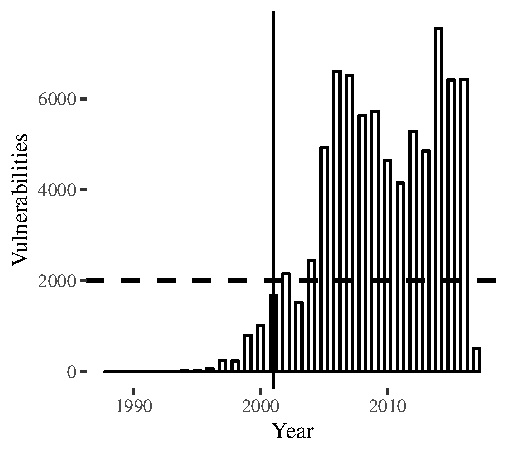
\includegraphics[width=\columnwidth]{nvd_vulns_year}
	\caption{NVD Vulnerability Count by Year}
	\label{fig:nvd_vulns_year}
\end{figure}
% stargazer(rtrunc)
% Table created by stargazer v.5.2 by Marek Hlavac, Harvard University. E-mail: hlavac at fas.harvard.edu
% Date and time: Sun, Feb 26, 2017 - 22:57:53
\begin{table}[!htbp] \centering 
	\caption{NVD Project Demographics} 
	\label{tab:nvd_demog} 
	\begin{small}
	\begin{tabular}{@{\extracolsep{5pt}}lccccc} 
		\\[-1.8ex]\hline 
		\hline \\[-1.8ex] 
		Statistic & \multicolumn{1}{c}{N} & \multicolumn{1}{c}{Mean} & \multicolumn{1}{c}{St. Dev.} & \multicolumn{1}{c}{Min} & \multicolumn{1}{c}{Max} \\ 
		\hline \\[-1.8ex] 
		CVECount & 10,622 & 4.311 & 5.241 & 2 & 49 \\ 
		logCVECount & 10,622 & 1.466 & 0.533 & 1.099 & 3.912 \\ 
		cvss\_score & 10,621 & 6.139 & 1.429 & 1.200 & 10.000 \\ 
		adherence & 10,621 & 4.678 & 1.007 & 0.225 & 6.532 \\ 
		cvss\_auth & 10,622 & 2.905 & 0.224 & 0.000 & 3.000 \\ 
		cvss\_access\_vector & 10,622 & 2.794 & 0.486 & 0.000 & 3.000 \\ 
		cvss\_access\_complexity & 10,622 & 2.577 & 0.409 & 0.000 & 3.000 \\ 
		cvss\_conf\_impact & 10,622 & 1.833 & 0.504 & 0.000 & 3.000 \\ 
		cvss\_integ\_impact & 10,622 & 1.902 & 0.467 & 0.000 & 3.000 \\ 
		cvss\_avail\_impact & 10,622 & 1.833 & 0.552 & 0.000 & 3.000 \\ 
		\hline \\[-1.8ex] 
	\end{tabular} 
		\end{small}
	
\end{table} 

\subsubsection{Estimation}

Combining the structural and measurement models we have defined with the CVSS data collected from the NVD database, we have the model definition, expressed in lavaan syntax: 

\begin{align*}
	SoftwareRisk =\sim cvss\_access\_vector \\ + cvss\_access\_complexity + cvss\_auth\\
	Outcomes =\sim logCVECount\\
	Outcomes \sim SoftwareRisk + Adherence + AssetValue\\
	Adherence =\sim adherence\\
	SoftwareRisk \sim Adherence\\
	AssetValue =\sim cvss\_conf\_impact\\
	 + cvss\_integ\_impact + cvss\_avail\_impact\\
\end{align*}		

\subsubsection{Model Fit}
SEM depends on the variances of the measured variables to be within an order of magnitude of each other. The base adherence and CVE Count metrics had variances two magnitudes larger than the other variables. We scaled adherence, and took the log of CVE Count to bring them within range of the other variables. The variation among the 22,000+ projects with exactly one vulnerability caused numeric problems for the estimation algorithm, and we elected to treat the group as outliers and drop them from consideration. We, further, excluded projects with 50 or more vulnerabilities as outliers (79 projects). After the exclusions, 10621 projects remained in the analyzed dataset. 

In terms of global fit, the fit index results for the initial NVD model were outside the range of standard fit criteria thresholds, as shown in the NVD column of Table \ref{tab:results_fit_all}, making the parameter estimates unreliable. 

\subsubsection{Re-specification}

Given that the fit results did not meet standard fit criteria thresholds, we consider a set of alternative measurement models, guided by our theoretical justification for each choice of measurement variable. We conduct an exploratory analysis, retaining the structural model, and altering the measurement model one measurement variable at a time. For each measurement variable in the Software Risk and Asset Risk factors, we drop a single measurement variable and re-estimate the model fit, e.g. estimating the initial model without cvss\_conf\_impact, then the initial model without cvss\_avail\_impact, etc. 

One of the re-specified models, dropping cvss\_access\_complexity from Software Risk, had global fit characteristics within the traditional fit criteria thresholds, as shown in the Respecified NVD column of Table \ref{tab:results_fit_all}. We present the parameter estimates for the Respecified NVD model in the results, and discuss the implications in Section \label{sec:case_nvd_discussion}.

\subsubsection{Reporting Results}
\label{sec:case_nvd_results}

Table \ref{tab:results_fit_all} presents the fit measure results for the NVD  and Respecified NVD models (as well as for the other case study models).

\begin{table*}
	\begin{center}	
		\caption{Global Fit Measures and Results}
			\label{tab:results_fit_all}
			\begin{tabular}{p{3cm}p{1cm}|p{2cm}p{2cm}p{2cm}p{2cm}p{2cm}}
				\\[-1.8ex]\hline 
				\hline \\[-1.8ex] 
				Fit Measure & Threshold & NVD	& Respecified NVD & CII	& Combined No Net  & Combined Net \\
				\hline \\[-1.8ex] 				
				Number of observations &  & $10621$  & $10621$ & $42$  & 49 & 19 \\				
				Model chi-square &  & $2759.88$ & 1005.6 & $42$ & 413.67 & 159.18\\				
				Model d.f. &  & $17$ & $12$ & $42$ & 105 & 105\\		
				Model p-value & $\leq 0.01$ & $0.0$ & $0.0$ & $42$ & $0.0$ & $0.0$\\
				RMSEA & $\leq 0.10$ &  $0.12$ &  $0.09$ & $42$ & 0.09 & 0.212 \\
				CFI & $> 0.90$ & $0.83$ & $0.93$  & $42$ & 0.889 & 0.616\\
				SRMR & $< 0.08$ & $0.08$ & $0.07$ & $42$& 0.12  & 0.178 \\
				\hline \\[-1.8ex] 				
			\end{tabular}
	\end{center}
\end{table*}

We report the estimated parameter values, unstandardized, for the Respecified NVD structural and measurement models in \ref{tab:results_nvd}.

\begin{table}
	\begin{center}	
		\caption{NVD Respecified Model Results}
		\label{tab:results_nvd}
		\begin{tabular}{l|rrrr}
				\\[-1.8ex]\hline 
				\hline \\[-1.8ex] 
			\textit{Latent Variables}:  & & & & \\  
			$\sim$ Measured variables& Estimate & Std.Err & z$-$value & $P(>|z|)$ \\
				\hline \\[-1.8ex]
			$SoftwareRisk =\sim$  & & & & \\                                   
			cvss\_ccss\_vctr   & 1.000 & &  & \\                             
			%initial: cvss\_ccss\_cmpl &  $-$2.19 &   0.235 &  $-$89.320 &   0.000\\
			cvss\_auth     &   $-$1.687  &  0.201  & $-$8.390   & 0.000\\
			$AssetValue =\sim$     & & & & \\                                    
			cvss\_conf\_mpct   & 1.000     & & & \\                       
			cvss\_intg\_mpct   & 0.797   & 0.011 & 70.746 &   0.000 \\
			cvss\_aval\_mpct  &  0.873   & 0.013 & 67.584   & 0.000 \\
			$Outcomes =\sim$    & & & & \\                                     
			logCVECount     &  1.000  & & & \\                          
			$Adherence =\sim$   & & & & \\                                      
			adherence    &     1.000        & & & \\                    
			Regressions:  & & & & \\  
			%& Estimate & Std.Err & z$-$value & $P(>|z|)$ \\
			$Outcomes \sim$         & & & & \\                                     
			SoftwareRisk   &  1.229 &   0.185 & 6.635 &   0.000 \\
			%Adherence       &  $-$2.84  &  6.829  &  -0.468  &  0.640\\
			AssetRisk     &   0.063  &  0.013  &  5.027 &   0.00\\
			$SoftwareRisk \sim$        & & & & \\                                  
			Adherence     &    0.039 &   0.005  &  8.618 &   0.000\\
			Covariances:  & & & & \\  
			%& Estimate & Std.Err & z$-$value & $P(>|z|)$ \\
			$AssetValue \sim\sim$          & & & & \\                                 
			Adherence      &  $-$0.017  &  0.005 &  $-$3.590 &   0.000\\
		\end{tabular}
	\end{center}
\end{table}

Interpreting the parameter estimates in terms of our hypothesized construct relationships, we have the following:
\begin{itemize}
	\item  Asset Risk is positively associated (0.063) with Security Outcomes, as hypothesized.
	\item Software Risk is positively associated (1.229) with Security Outcomes, as hypothesized. 
	\item Practice Adherence is positively associated (0.039) with Software Risk, contrary to what we hypothesized. 
\end{itemize}	
	  All three relationships were statistically significant. 

We present the standardized parameter estimates, and the residuals, in the context of the full structural and measurement models in Figure \ref{fig:nvd_model_respecified_estimates}. Circles represent the latent variables/factors of the structural model. Squares represent the measurement variables of the measurement model. Lines indicate relationships between variables. 

Single arrows from circles/factors to squares/measurement variables represent a factor `as measured by' a measurement variable relationship. The parameter estimate on these relationships represents the sign and magnitudue of the relative contribution of the measurement variable to the factor value.  

Single arrows from circles/factors to other circles/factors represent the sign and magnitude of the source latent variable's (bare side of line) effect on the target latent variable (arrowhead side of line). 

Dual arrows between circles/factors represent covariances between the factors. Dual arrows starting and ending at the same circle/factor or square/measurment variable indicate residual variance, the amount of variation in the data not explained by the model. 

Dashed lines indicate fixed estimates, set either by the modeler, or by the software. We have two examples of modeled fixed parameters: We specify the absence of a direct relationship between Asset Risk and Software Risk. We specify the absence of a direct relationship between Adherence and Outcomes, as we expect Adherence to affect Outcomes through being moderated by overall Software Risk. The remaining dashed lines are estimates fixed by the software, where it has estimated starting values in the course of solving the system of equations expressed by the model.  

\begin{figure*}
	\centering
	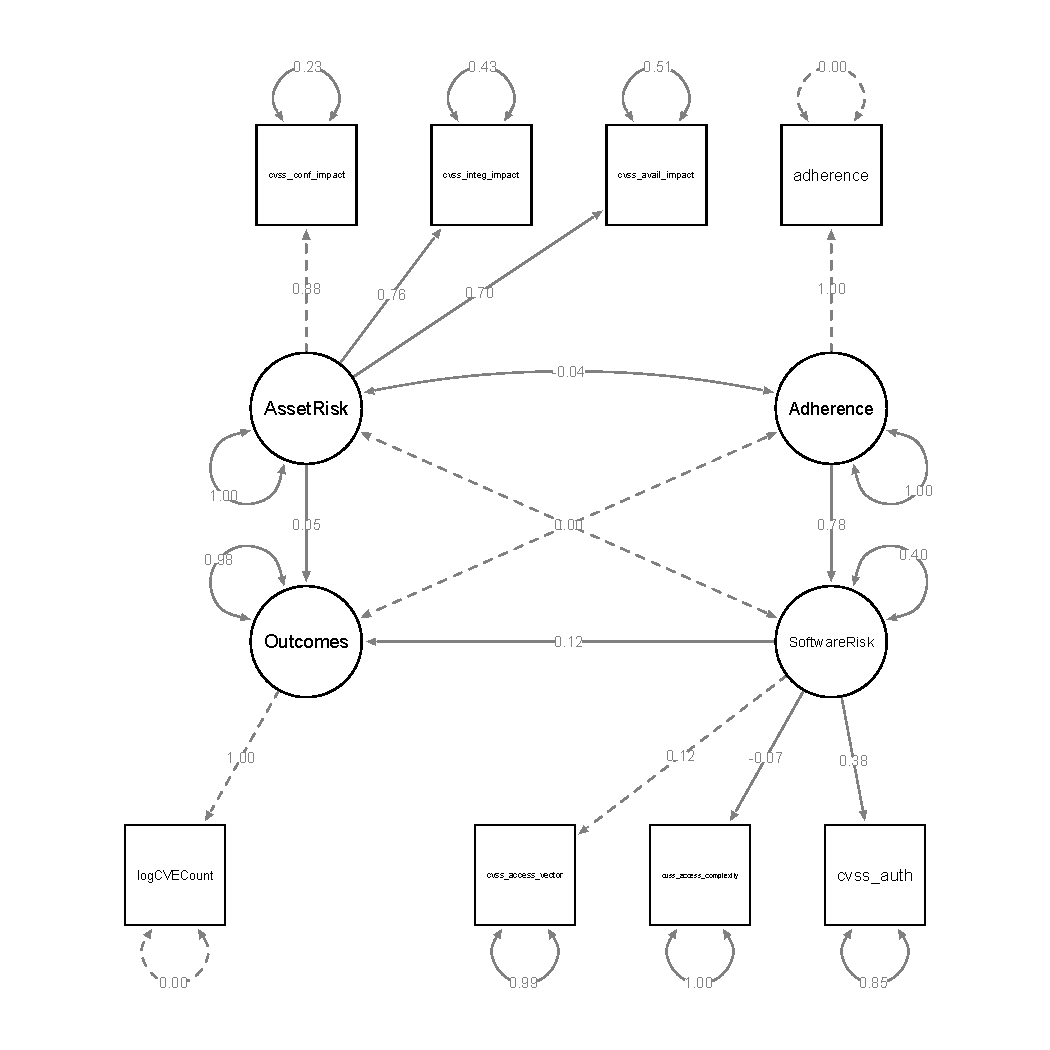
\includegraphics[width=\textwidth]{NVD_Respecified_SEM_Model.pdf}
	\caption{Respecified NVD Model}
	\label{fig:nvd_model_respecified_estimates}
\end{figure*}

We plot how the three impact risk scores change over time in Figure \ref{fig:nvd_vulns_impact}, and the CVSS access risk scores in Figure \ref{fig:nvd_vulns_auth}. 	
		
\begin{figure}
	\centering
	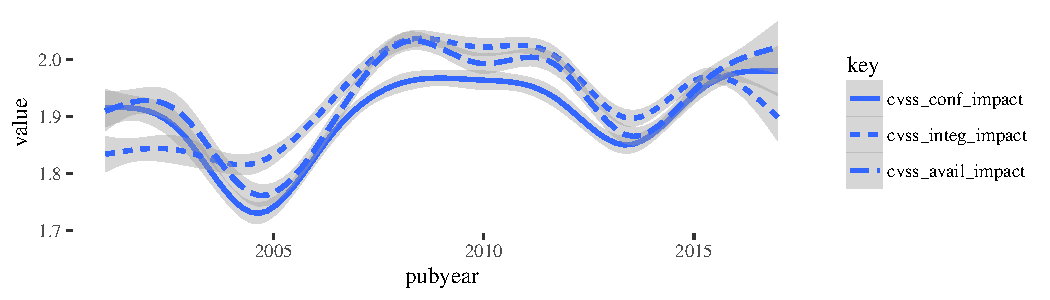
\includegraphics[width=\columnwidth]{nvd_cvss_impact}
	\caption{NVD CVSS Impact Risk by Year}
	\label{fig:nvd_vulns_impact}
\end{figure}

\begin{figure}
	\centering
	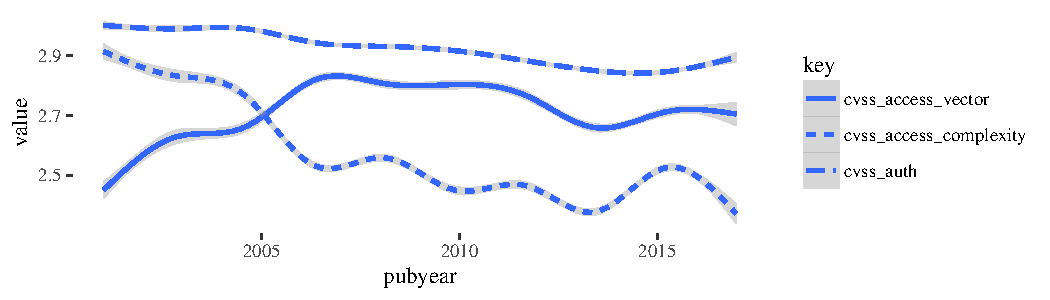
\includegraphics[width=\columnwidth]{nvd_cvss_auth}
	\caption{NVD CVSS Access Control Risk by Year}
	\label{fig:nvd_vulns_auth}
\end{figure}

For comparison, we ran a linear regression on logCVECount and all of the modeled measurement variables, results shown in Table \ref{tab:nvd_initial_regression}.

%stargazer(lm(logCVECount ~ cvss_access_complexity + adherence + cvss_access_vector + %cvss_auth + cvss_conf_impact + cvss_avail_impact + %cvss_integ_impact,data=rtrunc),style="asr")
% Table created by stargazer v.5.2 by Marek Hlavac, Harvard University. E-mail: hlavac at fas.harvard.edu
% Date and time: Fri, Mar 10, 2017 - 13:56:08
\begin{table}[!htbp] \centering 
	\caption{lm(logCVECount ~ cvss\_access\_complexity + adherence + cvss\_access\_vector + cvss\_auth + cvss\_conf\_impact + cvss\_avail\_impact + cvss\_integ\_impact)} 
	\label{tab:nvd_initial_regression} 
	\begin{tabular}{@{\extracolsep{5pt}}lc} 
		\\[-1.8ex]\hline \\[-1.8ex] 
		\\[-1.8ex] & logCVECount \\ 
		\hline \\[-1.8ex] 
		cvss\_access\_complexity & $-$0.038$^{**}$ \\ 
		adherence & 0.038$^{***}$ \\ 
		cvss\_access\_vector & $-$0.083$^{***}$ \\ 
		cvss\_auth & $-$0.172$^{***}$ \\ 
		cvss\_conf\_impact & 0.027 \\ 
		cvss\_avail\_impact & 0.115$^{***}$ \\ 
		cvss\_integ\_impact & $-$0.114$^{***}$ \\ 
		Constant & 2.075$^{***}$ \\ 
		\textit{N} & 10,621 \\ 
		R$^{2}$ & 0.030 \\ 
		Adjusted R$^{2}$ & 0.030 \\ 
		Residual Std. Error & 0.525 (df = 10613) \\ 
		F Statistic & 47.378$^{***}$ (df = 7; 10613) \\ 
		\hline \\[-1.8ex] 
		\multicolumn{2}{l}{$^{*}$p $<$ .05; $^{**}$p $<$ .01; $^{***}$p $<$ .001} \\ 
	\end{tabular} 
\end{table}

\subsubsection{Discussion}
\label{sec:case_nvd_discussion}
In our data, Adherence has a strong effect on Software Risk (0.68 standardized). Translated to the measurements we used, CVSS access vector metrics have been deteriorating over the last 15 years, and CVSS authentication metrics have been improving. One the one hand, the dramatic increase in web usage over the last 15 years correlates with the increase in network attacks represented by the access vector metric increase. On the other hand, the higher effort required by attackers over time is perhaps a positive reflection on the efforts of development teams to secure their software.  
 
We found small effects for both Asset Risk and Software Risk on Security Outcomes, with Software Risk having an effect (.13 standardized) roughly three times that of Asset Risk (0.05). We expect that the small (less than 15\%) effects of Asset Risk and Software Risk are due to the underlying measurement variables being incomplete accounts of the factors they measure; for example, the impact metrics say something about potential risks, but do not say anything about the environments in which the software runs, or about the kind of data maintained by the software in the contexts from which vulnerabilities were reported. Similarly, the software risk factors represented by CVSS access vector, and Authentication do not contain information on software size, churn, language, or the other factors that have been identified as contributing to security issues in software. 

Asset Risk is affected most strongly by the Confidentiality Impact measurement (.88 standardized), however the Integrity Impact (.76) and Availability Impact (.70) are in the same range and direction. Software Risk is affected most strongly by Authentication Risk (-0.44), although the sign of the parameter estimate is the opposite of our expectation. Lower Authentication Risk, meaning higher number of authentications required by attackers, may increase Software Risk through higher numbers of vulnerabilities being associated with software that implements access control, although further investigation is warranted. Given the single measurements, we have no information on the relative importance of the measurements for Adherence and Outcomes factors.

In general, the (standardized) residual variance values are higher than the .35 guideline established in Kline~\cite{kline2015principles}. The impact metric components of Asset Risk tend to have lower residuals as a group, suggesting that the that the three impact metrics are reasonably explained in terms of a common factor. The Access metrics have high residuals, suggesting that the Access metrics may not be reasonably explained in terms of a common factor. 

We have to account for why our initial theory and model did not predict that dropping the Access Complexity Risk factor from Software Risk would improve model fit. We consider three sources of failure: the metric, the measurement model, and the structural model.  One possible explanation is that Access Complexity is a poor measurement. The maintainers of the CVSS standard have acknowledged the overloaded nature of Access Complexity, stating that when it is applied it is impossible to tell if it is being used for user interaction from social engineering, from a race condition, uncommon configuration, attacker starting privileges, or anything else~\footnote{https://www.first.org/cvss}. However, each of the listed causes could be construed to be what we seek to measure for Software Risk. Version 3 of the CVSS (CVSSv3) scoring system includes a separate `User Interaction' metric to disambiguate between user-driven and software-driven reasons. In future work, we can update the measurement model to account for the updated CVSSv3 metrics. A second possible explanation is that measurement model is incorrect, via the Access Complexity metric being associated with the wrong factor, or a broader problem with assignments of metrics to factors. To test this notion, we fit the a model with Access Complexity associated with Asset Risk rather than Software Risk, but model fit was similarly poor. A third explanation is that our structural model is incorrect, either in the relationships between the factors, or in missing one or more factors with which Access Complexity could be associated. We put altering the structural model out of scope for the present work, but could investigate refinements of the structural model in future work. 

Per the descriptions of the metrics in Section \ref{sec:evaluation_nvd_selection_risk}, we view each of the metrics as measuring a property of the software that the development team can influence. Access Complexity Risk might be reduced through the addition, or refinement, of access control mechanisms. Alternatively, it might be increased by attacker discovery of alternate access paths.   Access Vector Risk might be reduced through care taken with validation of network inputs, or through greater care taken with implementation of network code, or increased through attacker path discovery. Authentication Risk might be reduced through stricter access controls, as with Access Complexity Risk, however the variables are not collinear in our data (as measured by Pearson's , Variance Inflation Factor). Authentication Risk might be increased, again by attacker discovery of alternative paths. Changes over time in each of the Access metrics may be due to development team efforts, or to attacker efforts, and we do not have the data here to distinguish between the two cases. We have assumed, in our modeling, that development team effort is the primary component for each metric. If attacker effort were the primary component, the metric should be modeled as part of Asset Risk.  If the three metrics we have were affected by different proportions of development team and attacker effort.

Our overall model data did not confirm Kaminsky's hypothesis that software quality is improving over time, with our adherence-over-time measure increasing Software Risk. However, we observed several counter-trends in the underlying data. We observed an improvement in CVSS Authentication Risk (Figure \ref{fig:nvd_cvss_auth}). On average, vulnerabilities are requiring more authentications over time, implying that development teams are putting an increasing amount of functionality behind access control.

We also observe from Figure \ref{fig:nvd_vulns_auth} that Access Complexity Risk has trended downward over time, in opposition to Authentication Risk and Access Vector Risk (Regressing Access Complexity Risk on adherence, controlling for the remaining measurement variables has a slope of -.09 for adherence, p-value $\textless$ 0.001). The trend suggests that, on average, over time, vulnerabilities are becoming more complicated for attackers, likely for a variety of causes, but potentially implying that access control is being implemented more frequently over time by development teams.

On the other hand, CVSS Access Vector Risk has increased in parallel to the decrease in Authentication Risk, indicating that vulnerabilities are increasingly prone to remote attacks from across the network.

 

\subsection{Core Infrastructure Initiative Case Study}

The Core Infrastructure Initiative was formed by the Linux Foundation to support critical elements of the global information infrastructure by identifying and funding projects in need of assistance~\footnote{https://www.coreinfrastructure.org/faq}. The CII team has developed a census of open source projects in potential need of assistance~\footnote{https://www.coreinfrastructure.org/programs/census-project}, as well as a program for measuring and rewarding compliance with good security practice~\footnote{https://bestpractices.coreinfrastructure.org/}.

\subsubsection{Data selection}
The CII census team has published the rationale behind their census and metrics ~\cite{wheeler2015open}, and has published their data and code on Github~\footnote{https://github.com/linuxfoundation/cii-census}. The 429 census records each contain data for one project deemed both important, and potentially at risk for security concerns, according to their criteria used by the CII team.

The project record contains descriptive data, e.g. project name and version, and security-relevant metrics, e.g. lines of code, contributor count, as well as an overall `risk index' based on the CII team's estimation of the importance of the metrics used to compute the index value.  Parallel to our translations of the CVSS metric score text to ordinal values, we translate the CII $fact\_activity$, $fact\_age$, $fact\_comments$, and $fact\_team\_size$ columns from text descriptions to ordinal values. We also parse the risk index components field to extract the ordinal ranks the CII team assigned each project for the risk index components: `Website points', `CVE Risk', `12 month contributors', `Popularity', `Language', and (network) `Exposure'. We now present our mapping of the CII metrics to our constructs.

\textbf{Asset Value}
The CII package\_popularity field contains Debian package popularity contest~\footnote{http://popcon.debian.org/} results, a measure of the frequency of use of each package on each system, aggregated to the relative usage of the package within the Debian ecosystem. We reason that paclage popularity is proportional to our theorized `Number of Machines'  metric, and, so, should be modeled as a component of Asset Value.

\textbf{Software Risk}
We model total\_contributor\_count, Contributor Risk, and total\_code\_lines as components of Software Risk, on the rationale that multiple studies (e.g. ~\cite{,camilo2015do,dashevskyi2016on}) have identified team size and code size as contributors to software vulnerability. The CII metrics direct\_network\_exposure and process\_network\_data, and potential\_privilege\_escalation are similar in concept to the CVSS Access metrics, and we, similarly, model them as components of Software Risk, theorizing that their values change based on design choices made by the software development team. We do not use the CII risk index measures, as they are composites, and we wish to examine the behavior of each of the index components.

\textbf{Adherence}
CII census data related to Adherence includes measurements of recent developer activity, and documentation effort. Developer activity is measured in the CII census data via a count of developers committing within the last year, twelve\_month\_contrib, and in terms of an ordinal categorical variable, fact\_activity, which we label TeamActivity. Documentation effort is measured in the CII census data via ordinal categorical variables in the risk index description for the amount and quality of comments, fact\_comments, which we label CodeComments, and by the presence of a website documenting the project, which we label WebsitePoints.

\textbf{Outcomes}
CII census data related to Outcomes includes a count of CVE vulnerabilities reported against the project since 2010. 

\textbf{Field choice notes}
The CII dataset contains a set of essentially co-linear fields, for example CVE Risk is translation of the CVE count since 2010 for the project into a categorical variable. We preferred counts to categorical values in initial field choices for the model.

\subsubsection{Data collection}

We retrieved the CII census data results file, current as of July 2016, from the project Github repository~\footnote{https://github.com/linuxfoundation/cii-census/blob/master/results.csv}. 

% stargazer(ciiraw)

% Table created by stargazer v.5.2 by Marek Hlavac, Harvard University. E-mail: hlavac at fas.harvard.edu
% Date and time: Sun, Feb 26, 2017 - 23:20:47
\begin{table*}[!htbp] \centering 
	\caption{} 
	\label{} 
	\begin{small}
	\begin{tabular}{@{\extracolsep{5pt}}lccccc} 
		\\[-1.8ex]\hline 
		\hline \\[-1.8ex] 
		Statistic & \multicolumn{1}{c}{N} & \multicolumn{1}{c}{Mean} & \multicolumn{1}{c}{St. Dev.} & \multicolumn{1}{c}{Min} & \multicolumn{1}{c}{Max} \\ 
		\hline \\[-1.8ex] 
		CVE\_since\_2010 & 428 & 7.262 & 26.142 & 0 & 422 \\ 
		twelve\_month\_contributor\_count & 346 & 98.965 & 491.693 & 0 & 3,768 \\ 
		total\_contributor\_count & 346 & 428.974 & 1,939.063 & 1 & 14,821 \\ 
		total\_code\_lines & 346 & 1,144,234.000 & 2,907,285.000 & 120 & 18,237,262 \\ 
		package\_popularity & 424 & 128,884.800 & 54,885.200 & 1 & 175,853 \\ 
		direct\_network\_exposure & 428 & 0.178 & 0.383 & 0 & 1 \\ 
		process\_network\_data & 428 & 0.152 & 0.359 & 0 & 1 \\ 
		potential\_privilege\_escalation & 428 & 0.058 & 0.235 & 0 & 1 \\ 
		risk\_index & 428 & 6.624 & 2.501 & 1 & 13 \\ 
		CVE & 428 & 7.262 & 26.142 & 0 & 422 \\ 
		RiskIndex & 428 & 6.624 & 2.501 & 1 & 13 \\ 
		TeamActivity & 428 & 1.509 & 0.988 & 0 & 3 \\ 
		CodeAge & 428 & 3.040 & 1.624 & 0 & 4 \\ 
		CodeComments & 428 & 2.231 & 1.773 & $-$1 & 5 \\ 
		TeamSize & 428 & 2.236 & 2.302 & $-$1 & 5 \\ 
		WebsiteRisk & 428 & 0.131 & 0.338 & 0 & 1 \\ 
		CVERisk & 428 & 1.044 & 1.266 & 0 & 3 \\ 
		ContributorRisk & 428 & 1.722 & 1.981 & 0 & 5 \\ 
		PopularityRisk & 428 & 1.808 & 0.494 & 0 & 2 \\ 
		LanguageRisk & 428 & 1.360 & 0.934 & 0 & 2 \\ 
		ExposureRisk & 428 & 0.558 & 0.777 & 0 & 2 \\ 
		DataRisk & 428 & 0.000 & 0.000 & 0 & 0 \\ 
		\hline \\[-1.8ex] 
	\end{tabular} 
	\end{small}
\end{table*}

\subsubsection{Estimation}


Combining the structural and measurement models we have defined with the metric data collected from the CII census, we have the model definition, expressed in lavaan syntax, in Figure \ref{tab:cii_model}.

\begin{align*}
SoftwareRisk =\sim  total\_contributor\_count\\ + ContributorRisk + total\_code\_lines\\ 
+ LanguageRisk + direct\_network\_exposure\\
 + process\_network\_data \\ 
+ potential\_privilege\_escalation + CodeAge \\
Outcomes =\sim  logCVECount \\
Outcomes \sim SoftwareRisk + Adherence + AssetValue \\
Adherence =\sim  TeamActivity + CodeComments + \\
	twelve\_month\_contributor_count + WebsiteRisk  \\
SoftwareRisk \sim  Adherence \\
AssetValue =\sim package\_popularity \\
AssetRisk ~~  Adherence\\
SoftwareRisk ~~ 0*AssetRisk\\
Adherence ~~ 0*Outcomes\\
\end{align*}

\subsubsection{Model Fit}
The initial model did not converge, after 678 iterations over the CII dataset.

We checked for collinearity, and eliminated twelve\_month\_contributor\_count, TeamSize, and ContributorRisk based on their collinearity on total\_contributor\_count. We eliminated ExposureRisk based on its collinearity with direct\_network\_exposure, and PopularityRisk based on its collinearity with package\_popularity.
 
\subsubsection{Re-specification}
Given that the initial model did not converge, we 
 
Table \ref{tab:results_fit_cii} presents the fit measure results for the final models of each case study. The baseline model, including all CII data fields, had poor fit indices (e.g. RMSE 0.237). We applied transformations and dropped fields from the model according to our expected theoretical relationships, but did not achieve significantly better model fit for the combinations we tested.

\subsubsection{Reporting Results}
Table \ref{tab:results_fit_all} presents the fit measure results for the CII case study (as well as for the other case studies). We report the estimated parameter values in \ref{tab:results_cii}.

In terms of global fit, the CII model was well outside the range of traditional fit criteria, as measured by the fit indexes. We did not conduct hypothesis tests for the model. 

\subsection{Combined CII and NVD data}
We observed that a subset of the CII census projects have vulnerabilities recorded in the NVD dataset, offering the opportunity to study the combination of measurement variables from the two datasets.  

\subsubsection{Data selection}
We began with the NVD and CII data, collected as previously described. 

\subsubsection{Data collection}
We intersected the two datasets based on the project name used in each dataset. Intersecting the 428 CII projects with the 10621 NVD projects yielded a set of 69 projects with all data for each project.

\subsubsection{Estimation}
We began with the aggregated fields from both datasets, and removed theoretically equivalent fields, preferring ordinal and ratio fields to categorical fields where we had a choice. For example, we chose the `package\_popularity' count over the `PopularityRisk' categorical variable. We evaluated model fit after each variable removal, addition, and transformation.

\subsubsection{Model Fit and Re-specification}
Through a series of experiments, evaluating model fit for the combined datasets, we obtained a `Combined' model with good global fit characteristics, see the `Combined No Net' column in Table \ref{tab:results_fit_all}.

\begin{align*}
	SoftwareRisk =\sim cvss\_access\_vector + cvss\_access\_complexity\\
	 + cvss\_auth + total\_code\_lines + TeamSize + LanguageRisk\\
	Outcomes =\sim  logCVECount \\
	Outcomes ~ SoftwareRisk + Adherence + AssetValue\\
	Adherence =\sim adherence + twelve\_month\_contributor\_count +\\ CodeComments + TeamActivity \\
	SoftwareRisk \sim  Adherence\\
	AssetValue =\sim cvss\_conf\_impact + cvss\_integ\_impact +\\ cvss\_avail\_impact + package\_popularity\\
\end{align*}

\subsubsection{Reporting Results}
To study how models behave for different projects, we selected a non-model variable, `process\_network\_data', to filter data for the model. We compared the performance of the model on projects that do not process network data against the model's performance in projects that process network data by filtering the data each way and applying the model.

\begin{table}
	\begin{center}	
		\caption{NVD-CII Combined, No Net Data}
		\label{tab:results_combined1}
		\begin{tabular}{l|rrrr}
			\\[-1.8ex]\hline 
			\hline \\[-1.8ex] 
			\textit{Latent Variables}: &  & Combined & No Net & \\  
			$\sim$ Measured variables& Estimate & Std.Err & z$-$value & $P(>|z|)$ \\
			\hline \\[-1.8ex]
			$SoftwareRisk =\sim$  & & & & \\                                   
			cvss\_ccss\_vctr   & 1.000 & &  & \\                             
			cvss\_ccss\_cmpl &  $-$0.36 &   0.286 & 1.243 &   0.214\\
			cvss\_auth     &   $-$0.065  &  0.056  & $-$1.17   & 0.244\\
			total\_code\_lns  &  6.232 &   2.572 &   2.423 &   0.015\\
			TeamSize        &  6.268   & 2.484   & 2.524   & 0.012\\
			LanguageRisk    &  0.148  &  0.413   & 0.357   & 0.721\\ 
			& & & & \\  
			$AssetValue =\sim$     & & & & \\                                    		
		    cvss\_conf\_mpct  &  1.000  &	&	&                  \\
		    cvss\_intg\_mpct  &  0.954  &  0.116 &   8.230  &  0.000\\
		    cvss\_aval\_mpct  &  0.896 &   0.122 &   7.361 &   0.000\\
		    package\_pplrty  &  0.458 &   0.464  &  0.987 &   0.324\\	
			& & & & \\  
			$Outcomes =\sim$    & & & & \\                                     
			logCVECount     &  1.000  & & & \\                          
			& & & & \\  
			$Adherence =\sim$   & & & & \\                                      
			adherence    &     1.000        & & & \\    
			
		    twlv\_mnth\_cnt\_  &  7.783  &  4.088  &  1.904 &   0.057\\
		    CodeComments    &  1.914  &  1.145  &  1.672  &  0.095\\
		    TeamActivity    &  1.386  &  0.842 &   1.646 &   0.100\\	
			                
			Regressions:  & & & & \\  
			%& Estimate & Std.Err & z$-$value & $P(>|z|)$ \\
			$Outcomes \sim$         & & & & \\                                     
			SoftwareRisk   &  3.365 &   1.635 & 2.058 &   0.040 \\
			Adherence       &  $-$1.559  & 1.526  &  $-$1.022  &  0.307\\
			AssetValue     &   $-0$.619  &  0.291  &  $-$2.125 &   0.034\\
			$SoftwareRisk \sim$        & & & & \\                                  
			Adherence     &    1.56 &   1.04  &  1.505 &   0.132\\
			Covariances:  & & & & \\  
			%& Estimate & Std.Err & z$-$value & $P(>|z|)$ \\
			$AssetValue \sim\sim$          & & & & \\                                 
			Adherence     &    $-$0.024 &   0.019  &  $-$.255 &   0.209\\
		\end{tabular}
	\end{center}
\end{table}


\begin{table}
	\begin{center}	
		\caption{NVD-CII Combined, Net Data}
		\label{tab:results_combined2}
		\begin{tabular}{l|rrrr}
			\\[-1.8ex]\hline 
			\hline \\[-1.8ex] 
			\textit{Latent Variables}: &  & Combined & No Net & \\  
			$\sim$ Measured variables& Estimate & Std.Err & z$-$value & $P(>|z|)$ \\
			\hline \\[-1.8ex]
			$SoftwareRisk =\sim$  & & & & \\                                   
			cvss\_ccss\_vctr   & 1.000 & &  & \\                             
			cvss\_ccss\_cmpl &  $-$0.224 &   0.272 & 0.822 &   0.411\\
			cvss\_auth     &   $-$0.1035  &  0.114  & $-$906   & 0.365\\
			total\_code\_lns  &  7.27 &   3.054 &   2.381 &   0.017\\
			TeamSize        &  8.448   & 3.092  & 2.732   & 0.006\\
			LanguageRisk    &  $-$0.976  &  0.645   & $-$1.513   & 0.130\\ 
			& & & & \\  
			$AssetValue =\sim$     & & & & \\                                    		
			cvss\_conf\_mpct  &  1.000  &	&	&                  \\
			cvss\_intg\_mpct  &  0.743  &  0.129 &   5.770  &  0.000\\
			cvss\_aval\_mpct  &  0.481 &   0.110 &   4.364 &   0.000\\
			package\_pplrty  &  0.378 &   1.099  &  0.344 &   0.731\\	
			& & & & \\  
			$Outcomes =\sim$    & & & & \\                                     
			logCVECount     &  1.000  & & & \\                          
			& & & & \\  
			$Adherence =\sim$   & & & & \\                                      
			adherence    &     1.000        & & & \\    
			twlv\_mnth\_cnt\_  &  3.852  &  0.951  &  4.051 &   0.000\\
			CodeComments    &  $-$0.486  &  0.353  &  $-$1.376  &  0.1695\\
			TeamActivity    &  0.123  &  0.352 &   0.350 &   0.726\\	
			
			Regressions:  & & & & \\  
			%& Estimate & Std.Err & z$-$value & $P(>|z|)$ \\
			$Outcomes \sim$         & & & & \\                                     
			SoftwareRisk   &  $-$6.314 &   4.033 & $-$1.566 &   0.117 \\
			Adherence       &  4.210  & 2.340  &  1.80  &  0.072\\
			AssetValue     &   $-$1.312  &  0.418  &  $-$3.142 &   0.002\\
			$SoftwareRisk \sim$        & & & & \\                                  
			Adherence     &    -0.003 &   0.035  &  -0.086 &   0.931\\
			Covariances:  & & & & \\  
			%& Estimate & Std.Err & z$-$value & $P(>|z|)$ \\
			$AssetValue \sim\sim$          & & & & \\                                 
			Adherence     &    $-$0.003 &   0.035  &  $-$.086 &   0.931\\
		\end{tabular}
	\end{center}
\end{table}

In terms of global fit, the Combined No Net model was inside or near the range of traditional fit criteria, as measured by the fit indexes. The Combined Net model was outside the traditional fit criteria on all measurements. In terms of the parameter estimates for our hypothesized  construct relationships, we have the following:
\begin{itemize}
	\item  Asset Value - Security Outcomes were negative ($-$0.619, $-1$1.312), contrary to our hypothesis. 
	\item Software Risk - Security Outcomes is positive (73.08), as hypothesized. 
	\item Practice Adherence is slightly postitively associated (0.045) with Software Risk 
\end{itemize}	
Only the Asset Risk-Outcome estimate was statistically significant.
